\subsection{Граф}

\begin{center}
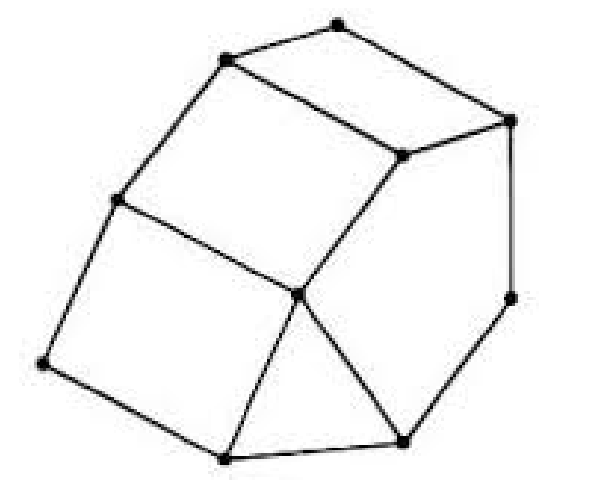
\includegraphics[width=0.4\textwidth]{par17graph.png}
\end{center}

Вершины = точки 

Ребра = линии, соединяющие некоторые пары вершин

Графы представляют объекты и связи между ними, например:

\begin{itemize}
    \item города и дороги
    \item люди и знакомства
    \item атомы и межатомные связи
\end{itemize}

\subsubsection*{Задача о Кенигсбергских мостах}

\begin{center}
    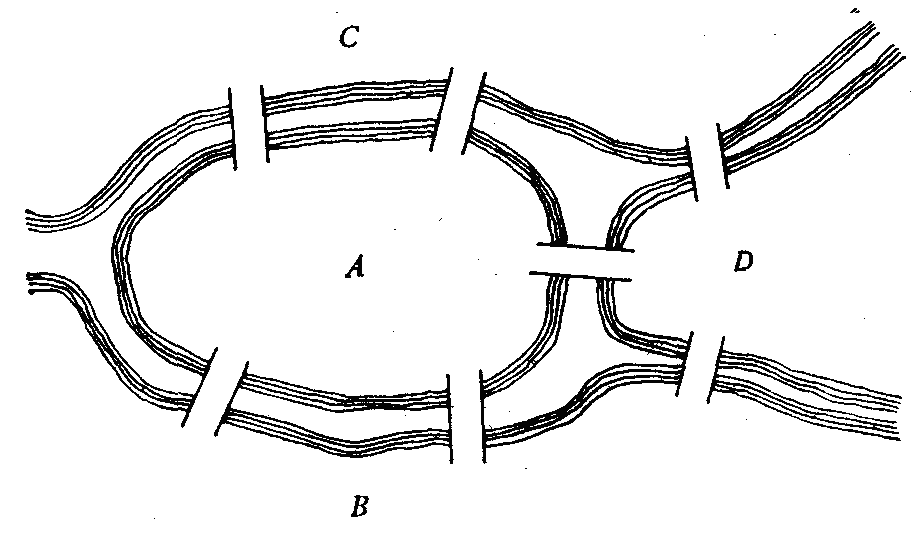
\includegraphics[width=0.7\textwidth]{par17kenig.png}
\end{center}

Можно ли обойти все Кенигсбергские мосты, пройдя только один раз через каждый из этих мостов?

Головоломке о мостах можно сопоставить граф (части города --- вершины, мосты --- ребра)

\begin{center}
    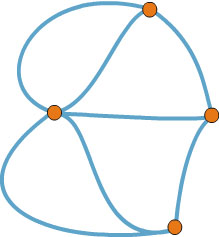
\includegraphics[width=0.2\textwidth]{par17kenig2.png}
\end{center}

Эквивалентная формулировка: можно ли <<обойти>> данный граф, пройдя по каждому ребру ровно один раз, и вернуться в исходную точку.

То есть существует ли последовательность ребер графа со следующими свойствами:
\begin{itemize}
    \item любые два соседних ребра имеют общую вершину;
    
    \item последнее ребро имеет общую вершину с первым ребром;
    
    \item каждое ребро графа встречается в последовательности ровно один раз.
\end{itemize}

Путем полного перебора несложно убедиться, что этот граф обойти нельзя.

Более общая задача:

\textbf{Задача.} (Эйлер, 1736)

Дан произвольный граф. Определить, можно ли его обойти в указанном выше смысле.

Исторически первый серьезный математический результат в теории графов.

\subsubsection*{Дома и колодцы (Головоломка о трех колодцах)}

В деревне три дома и три общих колодца. Можно ли протоптать тропинки так, чтобы от каждого дома к каждому колодцу вела тропинка и никакие две тропинки не пересекались?

Переведем на язык теории графов: 6 вершин, три из которых дома, другие три --- колодца; ребра соединяют каждую вершину-дом с вершиной-колодцем:

\begin{center}
    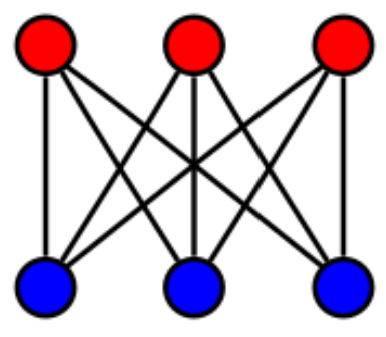
\includegraphics[width=0.2\textwidth]{par17k33.png}
\end{center}

Задача: можно ли перерисовать этот граф на плоскости так, чтобы никакие два ребра не пересекались.

Головоломка не имеет решения, но доказательство не тривиально, так как полный перебор тут бесполезен, поскольку способов нарисовать граф бесконечно много (будет позже).

Тип задач: изображение, или <<укладка>> графа так, чтобы выполнялись определенные свойства:

\begin{itemize}
    \item проектирование транспортных развязок (транспортные потоки разных направлений не должны пересекаться)
    \item печатных плат (не должны пересекаться проводящие дорожки)
\end{itemize}

\subsubsection*{Задача о деревенских свадьбах}

Третья задача, в отличие от двух предыдущих, является не индивидуальной, а <<массовой>> то есть в ее условии присутствуют параметры, которые можно менять.

В деревне живут несколько юношей и несколько девушек. Некоторые юноши знакомы с некоторыми девушками. Каждый юноша может пригласить на свадьбу только одну девушку, а каждая девушка может принять приглашение только от одного юноши. Нужно найти такое распределение юношей и девушек, чтобы каждый юноша знал хотя бы одну девушку, а каждая девушка знала хотя бы одного юноши. Требуется поженить максимально возможное число пар при условии, что женить можно только знакомые пары.

На языке теории графов:
\begin{itemize}
    \item вершины графа --- юноши и девушки
    \item ребра --- знакомые пары юноша-девушка
\end{itemize}

Требуется найти максимальное по размеру множество ребер, никакие два из которых не имеют общих вершин.

К такой же математической модели сводятся и другие задачи (например, задача о назначениях).

\subsubsection*{Задача о раскраске карты}

Дана политическая карта мира. Требуется раскрасить каждую страну в какой-либо цвет так, чтобы любые две граничащие между собой страны были раскрашены в разные цвета, использовав при этом минимально возможное число красок. (Две страны считаются граничащими, если их границы имеют общую линию, а не точку.)

На языке теории графов:
\begin{itemize}
    \item вершины графа --- страны,
    \item ребра соединяют граничащие страны.
\end{itemize}

Получаем

\subsubsection*{Задача о раскраске графа}

Дан граф. Требуется раскрасить вершины графа в минимальное число цветов так, чтобы любые две смежные вершины имели различный цвет.

\begin{center}
    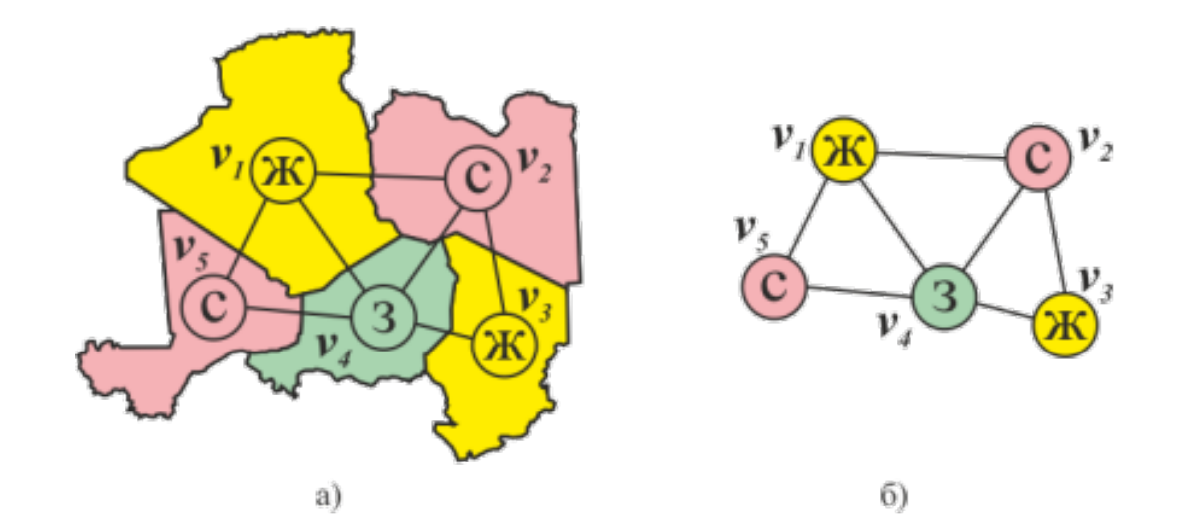
\includegraphics[width=0.9\textwidth]{par17color.png}
\end{center}